

\usepackage{graphicx}
\usepackage{titlesec}
\usepackage{geometry}
\usepackage{layout}
\usepackage{siunitx}
\usepackage{hyperref}
\usepackage{float}

\titleformat{\section}
	{\normalfont\fontsize{18}{19}\selectfont}{\thesection}{1em}{}
\titleformat{\subsection}
	{\normalfont\fontsize{13}{19}\selectfont}{\thesubsection}{1em}{}
\newcommand\headerquote[1]
	{\begin{center}\small\textit{#1}\end{center}}

\setlength{\footskip}{.6in}
\setlength{\textheight}{9.5in}
\setlength{\topmargin}{-1in}

\title{\bf Laboratory \#11 Proposal:\\ Physical Realizations of the Traveling Salesman Problem \vspace{-.5em}}
\author {\normalsize{Benjamin Huang \& Shiye SU}}
\date {\normalsize {Spring Semester, 2016} \vspace{-2em}}

%%END PREAMBLE%%

\begin{document}

\maketitle

\section{Background}

The initial inspiration for this idea came from a discussion about Markov Chain Monte Carlo (MCMC) algorithms. We both found the concept of MCMC algorithms very interesting, but we were struggling to find a way to incorporate them into our lab. Since MCMC algorithms are well known for finding quasi-optimal solutions to the Traveling Salesman Problem (TSP), we started to look for physical analogues to TSP that we could experimentally perform. This is how we came across the Ugajin paper about using an inverse diffusion process to optimize the renormalization solution described in Yoshiyuki and Yoshiki paper. 

\section{Experimental Design}

\begin{enumerate}
\item Can (a) the physical process of diffusion and (b) the chemotactic behaviour of C. elegans be exploited to find a good quasi-optimal solution to the traveling salesman problem? (Our standards for a `good' solution are based on comparisons to other quasi-optimal solutions (such as orthogonal gridding) and the optimal solution--we will explain this further). Furthermore, how does the computational time compare to other methods?

\item
\begin{itemize}

\item Yes, we expect that diffusive and chemotactic processes will be a better solution than arbitrary gridding, because cities of close proximity are naturally grouped together whereas arbitrary gridding is insensible to the city distributions. Computational times should be low for the scientific models and high for simulated annealing. 

\item No, diffusion and chemotaxis will do little to find a more optimal solution to the problem, as they point the solution search to a limited set, namely those that visit city groups together. Simulated annealing is more effective because it can potentially scan the entire solution spectrum. Further, processing times will make diffusion and chemotaxis unideal for traveling salesman applications, because image processing requires enormous computational power. (We are still thinking how we can quantify this)

\end{itemize}

\item \textbf{Background:} The traveling salesman problem is a classic problem in combinatorial optimization. It asks, for some spatial arrangement of cities, what is most efficient route (quantified by distance) that passes through each city? Currently, the solution to real-life, non-trivial arrangements is found by `computational bash', which is time and resource intensive. An active field of research is how we can find `quasi-optimal' solutions to the traveling salesman problem, which achieve a good compromise between an efficient route and computational time without the combinatoric explosion of testing every possible route.

\par
Our approach develops an idea we'll call \emph{orthogonal gridding}, which divides an arrangement of the cities first into four equal squares. We will call each unique arrangement a \emph{commonwealth}. Any single one of these four subdivisions, if it contains a city / cities, is considered a \emph{megalopolis} and treated as a unit. We then find the optimal route for visiting each megalopolis. Then the process is iterated: we treat each megalopolis as an independent commonwealth and apply orthogonal gridding to it, find the optimal solution, and subdivide further. In the final iteration, each megalopolis will be a single city, and we now construct the quasi-optimal solution to the entire problem by combining the smaller solutions. 

\begin{figure}[H]
\centering
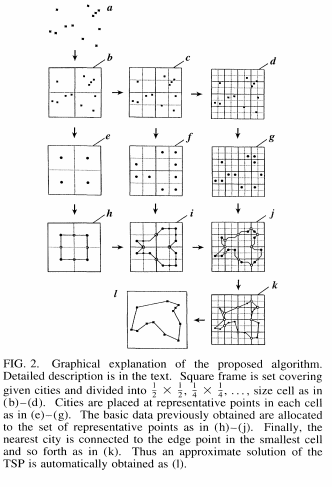
\includegraphics{AlgGroup}
\caption{Figure from the aforementioned gridding paper explaining their proposed algorithm. See the first bullet point in further readings for the original paper.}
\end{figure}

\par 
We want to investigate if two scientific phenomenon, diffusion and chemotaxis, can be used to find such a quasi optimal solution. Orthogonal gridding is unadaptable in the sense that it divides commonwealths the same way regardless of city distributions. However, we expect that diffusion and chemotaxis would more efficiently group cities into megalopolises. The general idea is that we take image sequences of diffusion and chemotaxis from each city until we have a homogenous plane of dye / overlapped trajectories. Each contiguous stretch of dye or of overlapped trajectories is a \emph{blob}. The image sequence is viewed in reverse. Each blob is considered a megalopolis, so the bifurcation of a single blob into two is analogous to one application of orthogonal gridding i.e. a division of the commonwealth into megalopolises. We then solve the traveling salesman problem for each blob. This entire iterative process we will call \emph{blobbing}.

\begin{figure}[H]
\centering
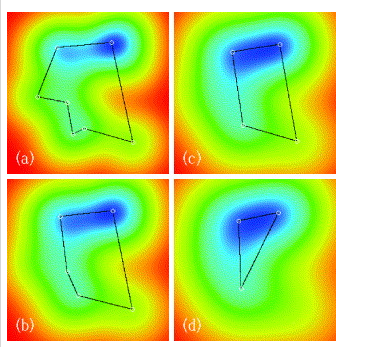
\includegraphics{Blob}
\caption{Figure of early stage \emph{blobbing} from the paper that describes the use of an inverse diffusion process. See the second bullet point in further readings for the original paper.}
\end{figure}

\textbf{General:} create 3 arrangements of 12 cities i.e. 3 commonwealths. One commonwealth has a trivial traveling salesman solution e.g. 12 cities arranged in a ring; the other two have nontrivial solutions. 

\par 
\textbf{Diffusion:} Create a board to which skewers can be attached in specific positions. For each commonwealth, each skewer will be fixed to the location of a city. We dip the skewer tips into a dye solution and touch the the skewer tips to a sheet of absorbent tissue e.g. kimwipe, filter paper. (Note: we may potentially use dye diffusing in water instead of through tissue, and may need to do some pre-tests to determine which is more effective.) Rest the tissue on some transparent platform so that a camera positioned from below can be used to capture image sequences of dye diffusing on paper. 

\par
\textbf{Chemotaxis:} Grow C elegans worms in \SI{50}{\milli \mol} NaCl solution. Pre make gradient agar plates of \SI{50}{\milli \mol} NaCl. Allow to set. For each commonwealth, stab holes in the agar plates for each city and fill hole with a dyed solution of higher concentration NaCl. Allow to set and diffuse to create radially symmetric gradients around each city. One city at a time, place a worm at the location of the city and acquire image sequences of the worm's chemotactic motion. Theoretically, the worm should migrate away from the city at which it is placed, seeking the \SI{50}{\milli \mol} NaCl in which is was raised. 

\par
\textbf{Computation:} The data we will be measuring specifically from the laboratory are image sequences. From diffusion, we will threshold the images so that the ink regions are clearly defined from the paper (no ink) regions. From chemotaxis, we are ultimately acquiring trajectory coordinates for the moving worm. We will define the spreading `blob' as a circle of radius $r(t)$ centred on each city, where $r$ worm's maximum displacement from the city at time $t$. For each commonwealth, we will load parallel arrays of 12 worms moving from their respective cities and see as time evolves, when two blobs merge. 


\par
We will run simulations for each commonwealth to determine the optimal solution, the solution found by orthogonal gridding, and the simulated annealing solution. These methods will be compared for accuracy and run time.

\item For what we will be measuring, see point above. Possible figures:
\begin{itemize}
\item Histogram of computational times 

\item Histogram of accuracy (distance of route)

\item For each megalopolis, schematic of how cities are partitioned into megalopolises through blobbing

\item Number of megalopolises vs. time, to show the bifurcations

\item Chemotaxis trajectory plot

\item Images of diffusion in action
\end{itemize}
\begin{figure}[H]
\centering
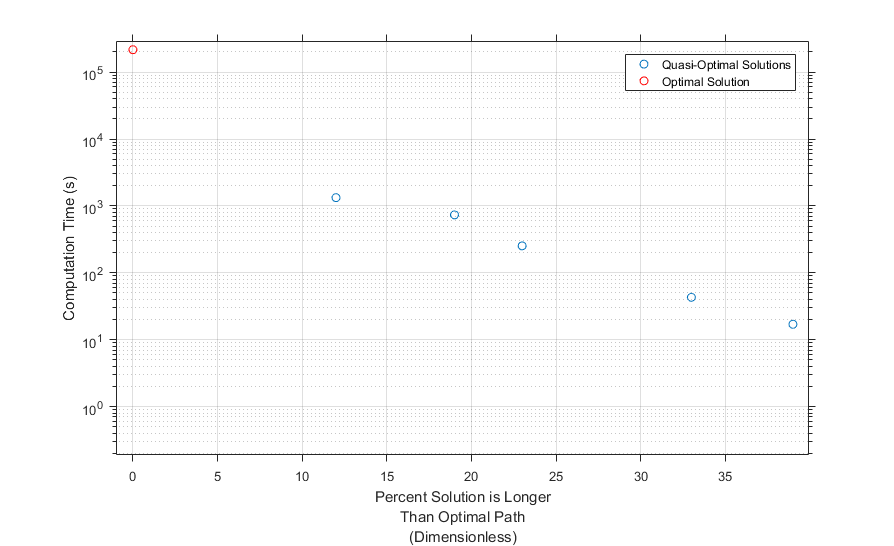
\includegraphics[width=1\textwidth]{FakeFig}
\caption{Example of a potential figure we could generate, comparing computational time with the percent that the path is longer than the optimal path.}
\end{figure}

\item Our two hypotheses represent somewhat opposing binaries. In the `successful' case that the blobbing method is effective, blobbing will divide up the commonwealth into megalopolises in an intuitive and effective manner, and we would have a high accuracy relative to other quasi-optimal methods. In `unsuccessful' case, it will not; particularly in the case of chemotaxis, the worms' unpredictable movement could cause unconventional blobbing divisions and a poor solution.\\\\
Links to further reading:
\begin{itemize}
\item\href{https://journals.aps.org/prl/pdf/10.1103/PhysRevLett.75.1683}{``New Method of Solving the Traveling Salesman Problem Based on Real Space Renormalization Theory''}
\item\href{http://www.sciencedirect.com/science/article/pii/S0378437101005714?np=y&npKey=0fa143539d8d6957c63ac58d4da7d077635c515d06bdb0de773f49508d699cc9}{``Method to solve the travelling salesman problem using the inverse of diffusion process''}
\item\href{http://iieom.org/ieom2014/pdfs/534.pdf}{``Worm Optimization: A novel optimization algorithm inspired by C. Elegans''}
\item\href{http://www.math.uwaterloo.ca/tsp/data/}{Database of Traveling Salesman Problems}
\end{itemize}

\end{enumerate}

\section{Logistics}

\begin{enumerate}
\item Perhaps the most difficult part of our lab will be working with \textit{C. elegans}. It will be hard to transfer them from the plates they grow on to our city plates and then quickly start taking data. This is important because we need them to start on top of specific ``cities'' and collect data as soon as they start moving. Furthermore, it may be hard to space the ``cities'' far enough apart to form an effective gradient that the \textit{C. elegans}. \\\\
Additionally, the sheer volume and complexity of computation involved in this lab may be difficult to conquer. Developing an efficient algorithm to determine when the diffusing points bifurcate could be especially difficult, not to mention possibly requiring a lot of computational power. Implementing simulated annealing in MATLAB is another difficulty that we will have to deal with--it may make more sense to use another language like Python. 
\item Our biggest points of failure have to do with computation. Even if \textit{C. elegans} are difficult to work with, we should be able to acquire enough data to do some analysis. The physical part of the diffusion process should not present any problem. The amount of computational work we have given ourselves is immense; however, if we achieve a few basic goals, then we would have no issue reducing the scope of our question. For example, we do not need to compare our results to the results of simulated annealing if simulated annealing proves too difficult to implement. This simply changes our methods of quantifying what is ``good''. Furthermore, by exploring two approaches, we always have a failsafe if we are unable to complete one. 
\item To perform the actual experiments, we will work together to perform them. In both of our experiments, it is important to start data collection immediately after the experiment has started. As such, one person will be in charge of setting up the experiment while the other one sets up the data collection. This will allow us to simultaneously start the data collection and the experiment, as well as move more rapidly than if we were both working independently. We anticipate having a lot of downtime as experiments run; we will use this time to analyze images and begin to write algorithms. For the computational work, we will develop algorithms for analyzing our data in tandem. The actual analysis will be evenly divided between us, as will the figure production. We will use GitHub for version control. 
\item We will need to prepare our gradient plates beforehand under the guidance of Jen. We need to build our apparatus for delivering dye to several points simultaneously, as well as test several dyes and \emph{terrains}. Furthermore, we need to be taught how to plate \textit{C. elegans} so that we are not relying on someone to plate them for us for the entire lab. 
\end{enumerate}

\end{document}